\subsection{Plot contrast against Fully-Associative Cache (Part3)}
\begin{figure}[H]
\centering
\begin{subfigure}{.48\textwidth}
  \centering
  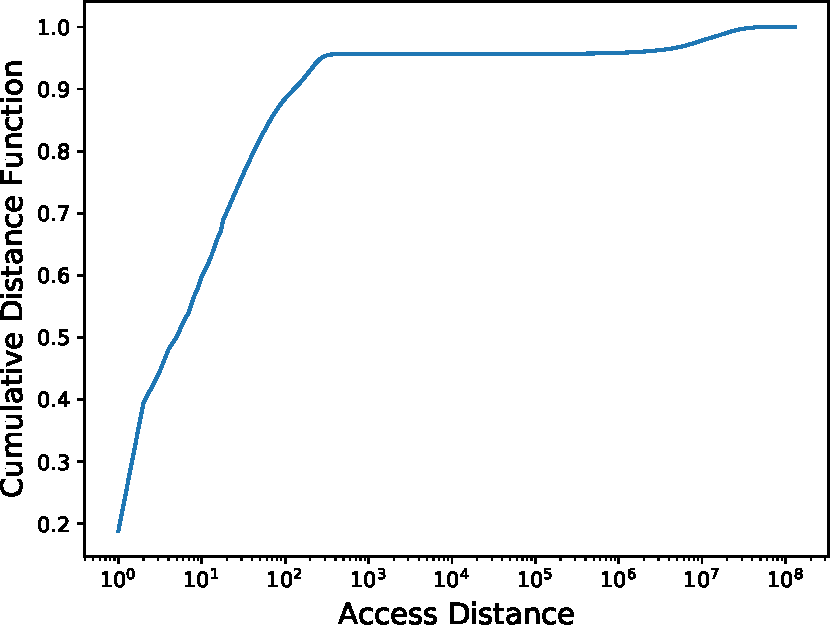
\includegraphics[width=\linewidth]{Q2addtrace1.pdf}
  \caption{CDF of access distance for misses of prog1.c}
  \label{fig:suba1}
\end{subfigure}%
\hspace{2mm}
\begin{subfigure}{.465\textwidth}
  \centering
  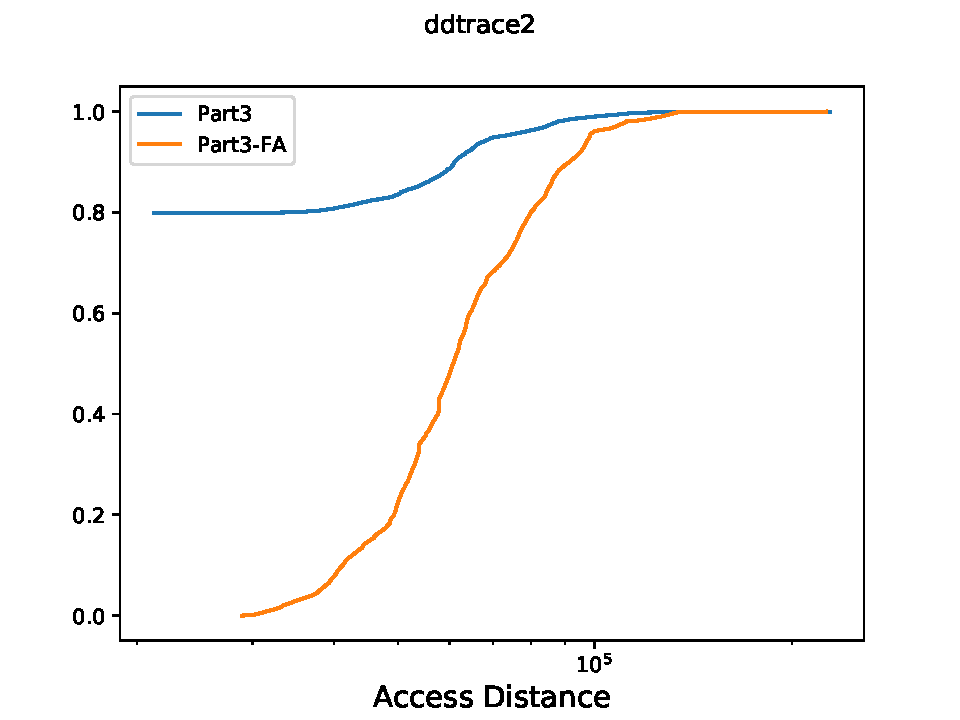
\includegraphics[width=\linewidth]{Q3addtrace2-test.pdf}
  \caption{CDF of access distance for misses of prog2.c}
  \label{fig:suba2}
\end{subfigure}
\label{fig:testa1}
\vspace{0.8in}
\begin{subfigure}{.48\textwidth}
  \centering
  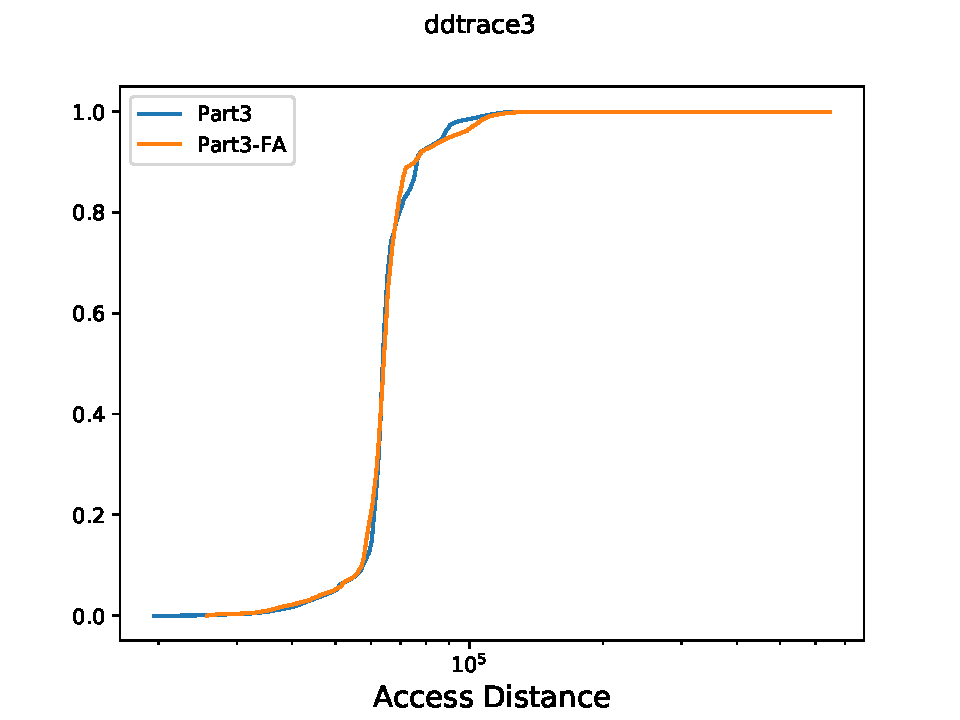
\includegraphics[width=\linewidth]{Q3addtrace3-test.pdf}
  \caption{CDF of access distance for misses of prog3.c}
  \label{fig:suba3}
\end{subfigure}%
\hspace{2mm}
\begin{subfigure}{.465\textwidth}
  \centering
  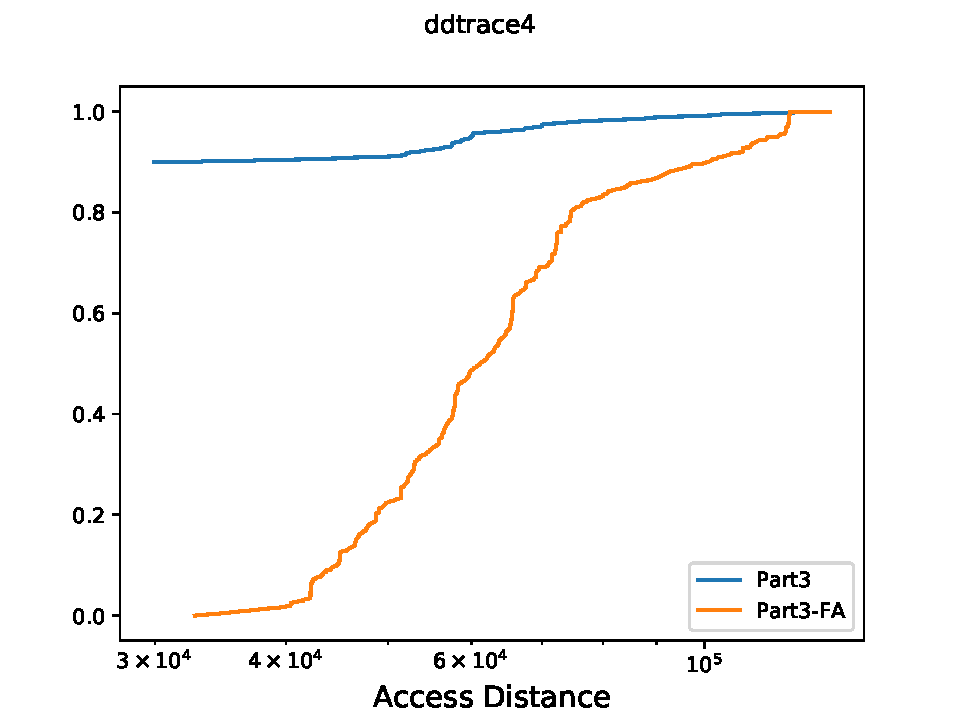
\includegraphics[width=\linewidth]{Q3addtrace4-test.pdf}
  \caption{CDF of access distance for misses of prog4.c}
  \label{fig:suba4}
\end{subfigure}
\caption{A comparison between the cdf-plots for miss traces with 16-way and Fully associative cache}
\label{fig:testa2}
\end{figure}